\documentclass[11pt]{article}

% Change "review" to "final" to generate the final (sometimes called camera-ready) version.
% Change to "preprint" to generate a non-anonymous version with page numbers.
\usepackage[]{acl}
\usepackage{times}
\usepackage{latexsym}

% For proper rendering and hyphenation of words containing Latin characters (including in bib files)
\usepackage[T1]{fontenc}
% For Vietnamese characters
% \usepackage[T5]{fontenc}
% See https://www.latex-project.org/help/documentation/encguide.pdf for other character sets

% This assumes your files are encoded as UTF8
\usepackage[utf8]{inputenc}
\usepackage{microtype}
\usepackage{inconsolata}
\usepackage{graphicx}
\graphicspath{{../../data/plots/}{../../data/plots/lgbm/}}

% If the title and author information does not fit in the area allocated, uncomment the following
%
%\setlength\titlebox{<dim>}
%
% and set <dim> to something 5cm or larger.

\title{Group 53 Progress Report:}


\author{Kelsey Rough, Rishi Dhanwantari, Rhea Gokhale \\
  \texttt{\{macid1,macid2,gokhaler\}@mcmaster.ca} }

%\author{
%  \textbf{First Author\textsuperscript{1}},
%  \textbf{Second Author\textsuperscript{1,2}},
%  \textbf{Third T. Author\textsuperscript{1}},
%  \textbf{Fourth Author\textsuperscript{1}},
%\\
%  \textbf{Fifth Author\textsuperscript{1,2}},
%  \textbf{Sixth Author\textsuperscript{1}},
%  \textbf{Seventh Author\textsuperscript{1}},
%  \textbf{Eighth Author \textsuperscript{1,2,3,4}},
%\\
%  \textbf{Ninth Author\textsuperscript{1}},
%  \textbf{Tenth Author\textsuperscript{1}},
%  \textbf{Eleventh E. Author\textsuperscript{1,2,3,4,5}},
%  \textbf{Twelfth Author\textsuperscript{1}},
%\\
%  \textbf{Thirteenth Author\textsuperscript{3}},
%  \textbf{Fourteenth F. Author\textsuperscript{2,4}},
%  \textbf{Fifteenth Author\textsuperscript{1}},
%  \textbf{Sixteenth Author\textsuperscript{1}},
%\\
%  \textbf{Seventeenth S. Author\textsuperscript{4,5}},
%  \textbf{Eighteenth Author\textsuperscript{3,4}},
%  \textbf{Nineteenth N. Author\textsuperscript{2,5}},
%  \textbf{Twentieth Author\textsuperscript{1}}
%\\
%\\
%  \textsuperscript{1}Affiliation 1,
%  \textsuperscript{2}Affiliation 2,
%  \textsuperscript{3}Affiliation 3,
%  \textsuperscript{4}Affiliation 4,
%  \textsuperscript{5}Affiliation 5
%\\
%  \small{
%    \textbf{Correspondence:} \href{mailto:email@domain}{email@domain}
%  }
%}

\begin{document}
\maketitle
% \begin{abstract}
% \end{abstract}

\section{Introduction}

The Swing Trading Strategy Analyzer tests if machine learning can help decide whether a setup is strong or weak for the moving-average pullback strategy specifically. A rule-based detector scans 4-hour bars across 76 stocks. It flags a setup when a stock is trending above the 50-bar simple moving average (SMA), then pulls back into its 20-bar exponential moving average (EMA), and then continues moving up.

The machine learning model gives each setup a probability of being successful. Every trade has a stop loss $1.5\times$ the average true range (ATR) under the entry and a profit target $3\times$ the ATR above it, with a 10-bar time limit. A success means the target is reached before the stop loss is hit and before the time limit is over. The model uses price action features and macro features influenced by the overall market. Features include news tone from GDELT and the VIX volatility index.

This problem is difficult for 3 reasons:
\begin{enumerate}
  \item There is a lot of noise in the market, so models can be wrong more often than not.
  \item Financial machine learning results can be inflated by leakage, where a feature accidentally uses information from after the trade decision.
  \item News data comes from a different source than the price data, so it has to be lined up carefully in time.
\end{enumerate}

Due to this, we are not aiming for a super accurate model. We are aiming for one that is correct and does not leak. The project is a success if filtering setups with the model gives better trading results than taking every setup the detector finds or than just buying and holding.
\section{Related Work}

Rhea will add her part today!!!

\section{Dataset}

You should write about your dataset here, following the guidelines regarding item 1. This section may be 0.5-1 pages. Depending on your specific dataset, you may want to include subsections for the preprocessing, annotation, etc.

\section{Features}

Each setup is one row of data with 21 features. They go straight into the tree models, with no embeddings or neural network. Stock prices vary a lot, so every price-based turns into a percentage or ratio. This is so all tickers are on the same scale.
 
\paragraph{Detector features:}
\begin{itemize}
  \item RSI
  \item ATR is percent of price
  \item how far the close price is above EMA20
  \item how far the close price is above SMA50
  \item trend strength is how far the EMA20 is above the SMA50
  \item if the signal came on the morning or afternoon bar
\end{itemize}

\paragraph{Technical features:} add information the detector doesn't use:
\begin{itemize}
  \item MACD line and histogram divided by the close price
  \item change in the MACD histogram over the 3 pullback bars, where positive means momentum is turning upward
  \item 20-bar volatility of log returns
  \item 5-bar vs. 20-bar volatility ratio, and above 1 means volatility is getting more intense
  \item signal bar volume compared to the average of the last 20 bars from the same session (the morning bar is 4 hours and the afternoon bar is 2.5 hours, so they can't be mixed)
  \item average relative volume during the pullback where low means a quiet dip and not heavy selling
\end{itemize}
 
\paragraph{Macro features:} overall market tone when the signal fires:
\begin{itemize}
  \item VIX: latest close, its 5-day change, and its distance from its 20-day average
  \item GDELT, from 72 hours before the signal bar closes:
  \begin{itemize}
    \item average news tone
    \item average Goldstein score (a scale from conflict to cooperation)
    \item average tone of U.S.\ events
    \item change in tone (last 24 hours vs. the last 48 hours)
    \item news volume ratio (last 24 hours vs. the last 48 hours)
  \end{itemize}
\end{itemize}
 
\paragraph{Leakage prevention:} 
\begin{itemize}
  \item Each feature table saves the timestamp of the newest data it used, and a check makes sure none of them are later than the signal bar's close.
  \item The VIX daily close only counts as available from the next day.
  \item A GDELT hour only counts once it is fully over.
  \item We also run a truncation test. It cuts the raw data off right after random setups, rebuilds the features, and checks that values for earlier setups do not change. If they did, the feature would be using future data.
  \item Separate checks were run for the technical and macro features.
\end{itemize}
 
\paragraph{Feature selection.} We also tested relative strength features against SPY: a 20-bar relative return, a short-term relative return, and a rank across tickers. They didn't improve the walk-forward results, so we left them out. The effect of each feature group is shown in the ablation in the Implementation section.

\section{Implementation}

Describe your model and implementation here. Refer to item 4. This may take around a page.

\section{Results and Evaluation}

\paragraph{Splitting:} Setups are sorted by signal time. The last 20\% (268 setups) is the final test set and the first 80\% (1,038 setups) is used for training. A random split would let the model learn from setups that happen at the same time as the test setups, which inflates results. We also use a 3-day embargo, so training trades have to close at least 3 days before the test window starts. This means trade outcomes do not overlap with the test period.

\paragraph{Cross-validation:} Hyperparameters are only tuned on the training set, they use expanding-window walk-forward folds.
\begin{itemize}
  \item The training data is split into 5 chunks in time order.
  \item Fold $k$ trains on chunks 1 to $k$ and validates on chunk $k+1$, with the same embargo.
  \item Settings are picked by the average PR-AUC across the folds.
\end{itemize}
To have a stronger check, a full walk-forward run retrains the model across 8 time windows over the whole history and scores each window on data it has not seen.

\paragraph{Classification metrics:} Only about 21\% of test setups are wins, which makes it inaccurate. These get reported:
\begin{itemize}
  \item precision, which is the amount of predicted wins that actually win
  \item recall, which is the share of actual wins that the model predicts as wins
  \item PR-AUC, compared against the 21\% base rate
  \item ROC-AUC, 0.5 means random ranking
  \item TSS (true skill statistic), which is recall minus the false positive rate, where 0 means no skill
\end{itemize}

\paragraph{Trading metrics:} Trades measured in R, which is profit in units of the risk taken. A full win is $+2$R and a full stop out is $-1$R. We report win rate, average R per trade, Sharpe ratio and max drawdown. To compare with buy-and-hold percentage returns, each trade is assumed to risk 1\% of the account.

\paragraph{Baselines:}
\begin{itemize}
  \item buy and hold SPY and QQQ
  \item equal weight buy and hold of all 76 tickers
  \item the unfiltered detector takes every setup
\end{itemize}
The unfiltered detector is the main baseline. If the model does not beat it, the model does not add value.

\paragraph{Results so far:} Table~\ref{tab:test} shows the test set results. Neither model decides winners against losers better than chance, and both have precision almost equal to the base rate.

\begin{table}[t]
  \centering
  \small
  \begin{tabular}{lcc}
    \hline
    \textbf{Test set (268 setups)} & \textbf{XGBoost} & \textbf{LightGBM} \\
    \hline
    ROC-AUC   & 0.49   & 0.46   \\
    PR-AUC    & 0.21   & 0.20   \\
    Precision & 21.1\% & 18.8\% \\
    Recall    & 26.8\% & 26.8\% \\
    TSS       & 0.004  & $-0.04$ \\
    \hline
  \end{tabular}
  \caption{Classification result for the final test set. The base rate is 20.9\% wins.}
  \label{tab:test}
\end{table}

While tuning, the best settings scored about 0.30 PR-AUC, compared to fold base rates of 0.20 to 0.27. This looked like a small edge, but it disappeared on the test set. Picking the best of 24 (XGBoost) or 36 (LightGBM) settings on only about 1,000 rows gives a score that is good but only because of luck. Both models also picked the largest minimum leaf size, which is what tuning tends to do when there not much of a real pattern to find.

The walk-forward results are similar (Figure~\ref{fig:wf}). Across both models and all the feature sets, ROC-AUC is between 0.49 and 0.53, and every 95\% confidence interval has 0.5. ROC-AUC for individual windows ranges from 0.35 to 0.74 where there s no steady trend, which indicates luck and not a skill that will hold over time.

\begin{figure}[t]
  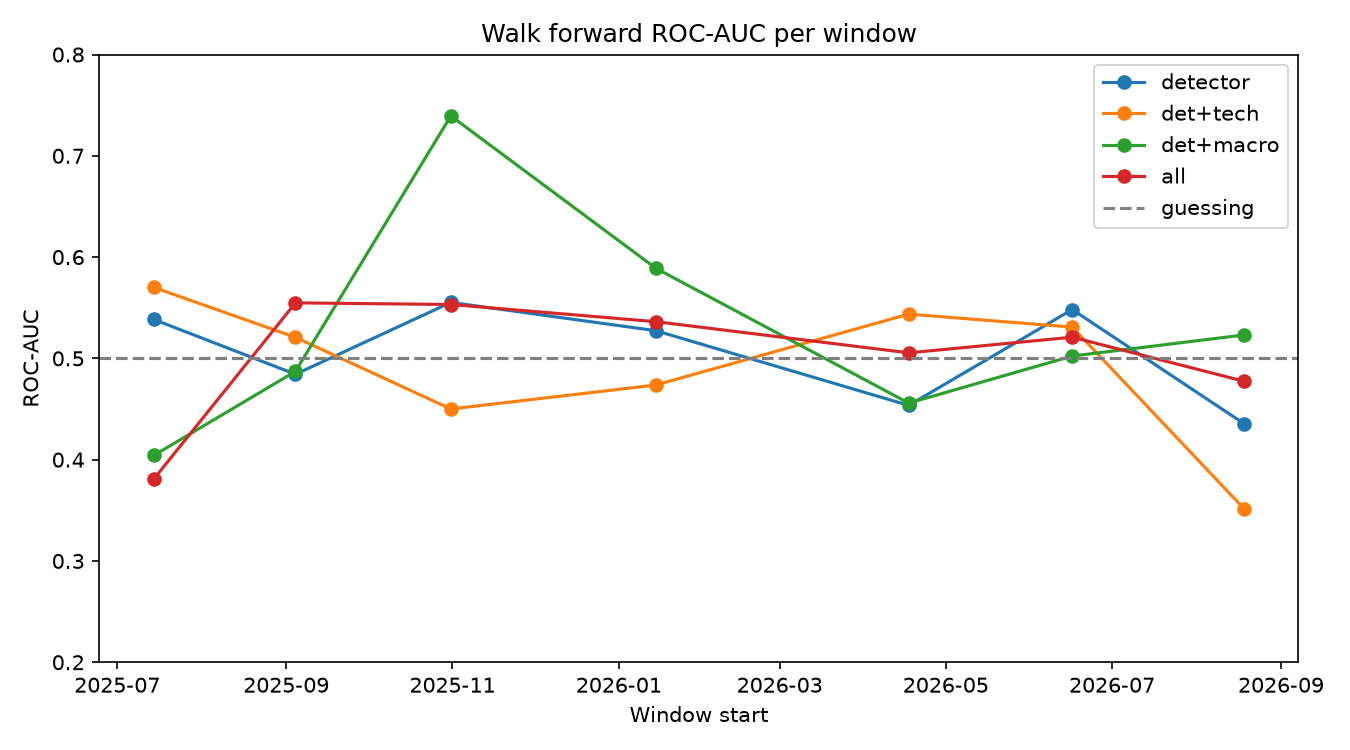
\includegraphics[width=\columnwidth]{wf_roc_by_window_gall_compare.png}
  \caption{Walk-forward ROC-AUC for each time window and feature set, the values stay close to 0.5.}
  \label{fig:wf}
\end{figure}

Table~\ref{tab:backtest} shows the backtest over the approximately 90-day test window.
\begin{itemize}
  \item The XGBoost filter took 71 of the 268 setups.
  \item It returned $+2.2$\% (Sharpe 0.43), compared to $+4.1$\% (Sharpe 0.47) for the unfiltered detector.
  \item It reduced the max drawdown from 18.8\% to 7.8\%, mostly because it took fewer trades.
  \item The equal weight buy and hold returned $+9.9$\% (Sharpe 2.11), which is higher than both.
\end{itemize}

\begin{table}[t]
  \centering
  \small
  \setlength{\tabcolsep}{3pt}
  \begin{tabular}{lrrrr}
    \hline
    & \textbf{Return} & \textbf{Sharpe} & \textbf{Max DD} & \textbf{Trades} \\
    \hline
    SPY hold            & $+3.5$\% & 0.91    & 3.5\%  & --  \\
    QQQ hold            & $-4.5$\% & $-0.53$ & 10.3\% & --  \\
    Equal-wt hold       & $+9.9$\% & 2.11    & 3.3\%  & --  \\
    Unfiltered detector & $+4.1$\% & 0.47    & 18.8\% & 268 \\
    XGBoost ($p \geq 0.5$) & $+2.2$\% & 0.43 & 7.8\%  & 71  \\
    \hline
  \end{tabular}
  \caption{Backtest over the final test window. Each trade risks 1\% of the account. The equal weight hold is rebalanced every day.}
  \label{tab:backtest}
\end{table}

The model's picks earned a little more per trade than all the setups on the test set, 0.041R compared to 0.027R (Figure~\ref{fig:equity}). With ROC-AUC around 0.5, it is likely that the difference is due to noise. Total R was also lower for the model (2.9R vs 7.2R) because it took less trades.

\begin{figure}[t]
  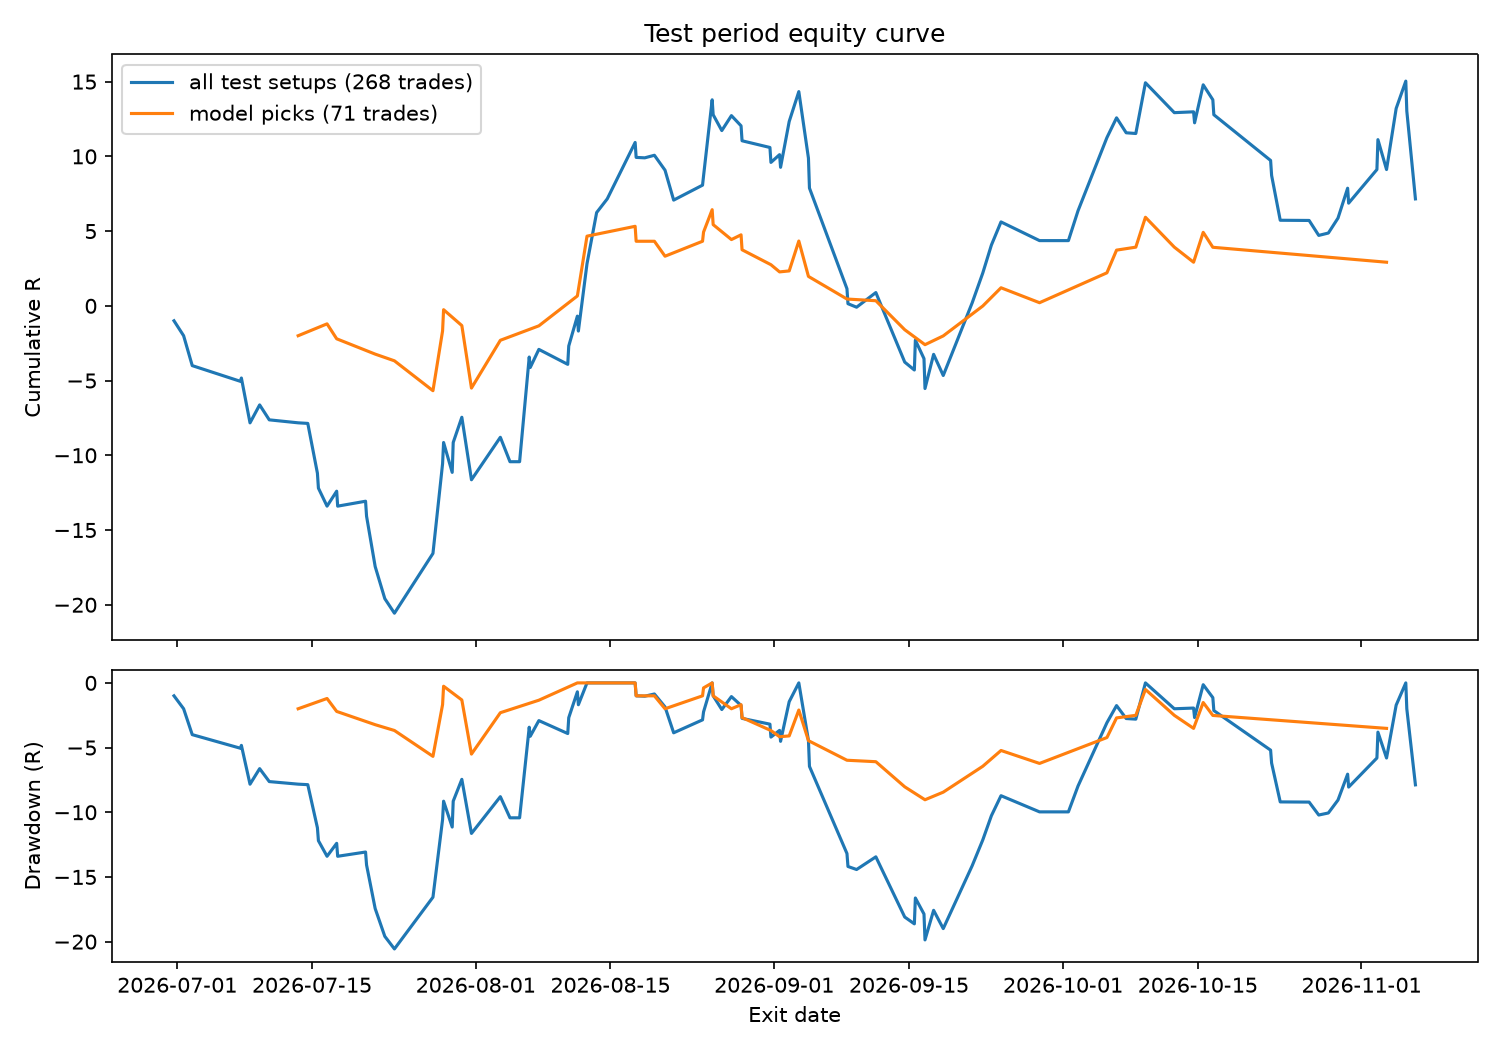
\includegraphics[width=\columnwidth]{equity_curve.png}
  \caption{Cumulative R for model filtered trades compared to all of the detector setups.}
  \label{fig:equity}
\end{figure}

Over the full history, the unfiltered detector averaged $+0.157$R per trade over 1,315 trades. This suggests the pullback pattern is mildly positive on its own, but our current features do not predict which setups will work.
\section{Feedback and Plans}

Write about your plans for the remainder of the project. This should include a discussion of the feedback you received from your TA, and how you plan to improve your approach. Reflect on your implementation and areas for improvement. Refer to item 6. This may be around 0.5 pages.

\section{Template Notes}

You can remove this section or comment it out, as it only contains instructions for how to use this template. You may use subsections in your document as you find appropriate.

\subsection{Tables and figures}

See Figure~\ref{fig:experiments} for an example of a figure and its caption.


\begin{figure}[t]
  \includegraphics[width=\columnwidth]{example-image-golden}
  \caption{A figure with a caption that runs for more than one line.
    Example image is usually available through the \texttt{mwe} package
    without even mentioning it in the preamble.}
  \label{fig:experiments}
\end{figure}

\begin{figure*}[t]
  \includegraphics[width=0.48\linewidth]{example-image-a} \hfill
  \includegraphics[width=0.48\linewidth]{example-image-b}
  \caption {A minimal working example to demonstrate how to place
    two images side-by-side.}
\end{figure*}


\subsection{Equations}

An example equation is shown below:
\begin{equation}
  \label{eq:example}
  A = \pi r^2
\end{equation}

Labels for equation numbers, sections, subsections, figures and tables
are all defined with the \verb|\label{label}| command and cross references
to them are made with the \verb|\ref{label}| command.
This an example cross-reference to Equation~\ref{eq:example}. You can also write equations inline, like this: $A=\pi r^2$.


% \section*{Limitations}

\section*{Team Contributions}

Write in this section a few sentences describing the contributions of each team member. What did each member work on? Refer to item 7.


% \appendix

% \section{Example Appendix}
% \label{sec:appendix}

% This is an appendix.

\end{document}
